\chapter[SCP-036 雅兹迪信徒的重生朝圣之旅]{
    SCP-036 The Reincarnation Pilgrimage of the Yazidi (Kiras Guhorîn)\\
    SCP-036 雅兹迪信徒的重生朝圣之旅
}

\label{chap:SCP-036}

\begin{figure}[H]
    \centering
    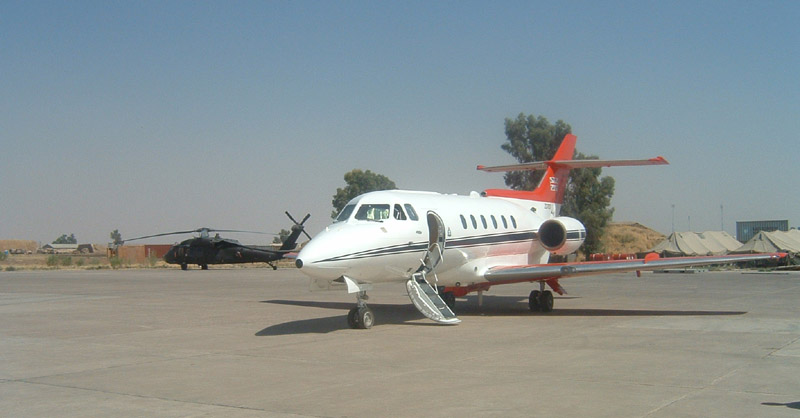
\includegraphics[width=0.5\linewidth]{images/SCP.036.jpg}
    \caption*{一架朝圣航班正在等待起飞}
\end{figure}

\bb{项目编号:}SCP-036

\bb{项目等级:}Safe

\bb{特殊收容措施:}每一年,一支机动特遣队将会从位于{[}数据删除]的收容指挥部02(Containment Command-02)派出到22A站点(Site-22A)来守卫位于当地的飞机跑道和机场。所有的市民設施将在9月23日下午0400进行非基金会人员的清除,并且他们不允许在在第二天日出之前回来。在10月1日,所有的市民又必须要在日出之前进行撤离,并且不允许进入22A站点直到“朝圣航班”归来。

由“抵达航班”所运来的乘客在等待登上“朝圣航班”时,只能由安全等级3以上的研究员对于乘客进行安检。

\bb{描述:}SCP-036包括了一个它的所在地,22A站点(一个位于北伊拉克摩苏尔山区的小机场)和22B站点(在22A站点等级的乘客的最终目的地)。036的关键组件有:

\begin{itemize}
\item “抵达航班” - 一架在9月23日日落之前不久抵达的客机(每一年都会在制造厂商和外观上有所不同)。它将会在离22A站点30-40km处时在雷达上出现。当它降落之后,“朝圣者”将会从飞机上下来并且进入候机大楼。没有任何机组人员曾离开过飞机。观察只发现了一名戴着面具的飞行员和一名助理飞行员。这架飞机在朝圣者都下机之后将会很快地离去,并且从不等待起飞许可,同样地也不在降落的时候表明身份。
\item “朝圣者” - 从飞机上下来的有着雅兹迪信仰的乘客们,他们都说他们正在去“kiras guhorîn”。每一年他们都接受检查并且确认为是在上一年之中死去的有着雅兹迪信仰的人们。这是通过出生证明、带照片的身份证、特殊知识的问题、并且在可能的情况下,进行指纹鉴定来进行调查的。他们之中的大部分都被认为是友好的并且温和的,虽然他们之中的大部分都吞吞吐吐不愿意给出kiras guhorîn的细节。在过去的情况里,他们都表现得无法辨认出朋友和家人或者只能保留一些在短期记忆时间内可以保留的回忆。在九月23日下午的最后时间,大部分的朝圣者们都会开始强调他们即将开始的朝圣是多么地重要。在那时候,他们将会开始登上“朝圣航班”并且出发,最后再也没有被人所见过。
\item “朝圣航班” - 一架由基金会人员所提供的用以运输“朝圣者”的客机,它是由一群由良好训练的雅兹迪圣职者组成的机组人员来进行操控的。这群机组人员从不能很好地描述有关于朝圣者的细节和究竟什么是kiras guhorîn。在飞机上的SCP装备能够在光学层面上运作,但是每一年都只能稍微增加我们对于这些朝圣者的认识。虽然这架飞机消失了7天,但是机组人员和记录的数据只能得出过去了数个小时的结论。数日的时间就这样从时间计算工具和摄像机上消失了,虽然从没有观察到任何的异常现象。飞机从雷达上消失,并且在离22A站点大约50-60的距离处就与地面人员失去了视觉联系,直到它在10月1日的日出时重新回归。
\item 22B站点 - “朝圣航班”的最终目的地。那是一个仅有一座建筑物和一条跑道组成的小机场,坐落于坐标{[}数据删除]。它只能被“朝圣团”和飞机上的摄像设备所记录。它并没有出现在卫星图像上,并且步行抵达该地点的尝试也失败了,有一次甚至带来了损失惨重的结果。摄像机在对于该地点聚焦时会出现问题,因为从地面蒸腾而起的热量通常会在飞机数十米远处的物体上造成类海市蜃楼的视觉效果。一次由SCP侦察机在朝圣活动前数周对于该地点的掠影只发现了未曾开发过的大地和一个类似于远古石雕像的物体。在20世纪90年代,机动特遣队Sigma-4想要在朝圣期间抵达22B站点。他们一接近,通信就此中断了,并且他们再也没有被听说过。在这朝圣的7日期间,不推荐任何其他的探索活动。
\end{itemize}

\begin{figure}[H]
    \centering
    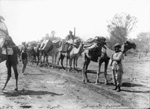
\includegraphics[width=0.3\linewidth]{images/SCP.036.2.jpg}
    \caption*{在朝圣开始前不久的雅兹迪圣职者}
\end{figure}

最初,那些说库尔德语的雅兹迪信徒秘密地进行着他们的朝圣活动。从东方而来的朝圣者被戴着面具的武装守卫送到雅兹迪圣职者那里,接下来的事情他们解释道那些圣职者将会将这些朝圣者带向西方,带到他们的“冥土之地”,在那里这些朝圣者们将会重新等待“重生”为雅兹迪信徒。词语“kiras guhorîn”,在库尔德语的字面意思就是“换装”,用于描述对地位较低的雅兹迪信徒灵魂所经历的重生的信仰。虽然真实的朝圣活动一直在秘密进行,一个象征意义的朝圣和“kiras guhorîn”每一年都在此时由其他的雅兹迪信徒进行着。

在20世纪60年代,库尔德人和穆斯林的占地行为、土耳其人的攻击和伊斯兰伊拉克政府颁布的惩罚性法令,限制了雅兹迪信徒的迁移和传统。在那段时间之中,基金会进行了介入并以一条准许基金会飞机不受限制地降落于该地机场的有利条款的形式提供援助。几乎是与此同时,携带着朝圣者的神秘飞机自东而来,降落在了当地的机场,同时在目的地也出现了那个令人难以捉摸的机场。
